\documentclass[aps,prd,twocolumn,showpacs,superscriptaddress,groupedaddress,nofootinbib]{revtex4}  % for review and submission
%\documentclass[aps,preprint,showpacs,superscriptaddress,groupedaddress]{revtex4}  % for double-spaced preprint
\usepackage{graphicx}  % needed for figures
\usepackage{dcolumn}   % needed for some tables
\usepackage{bm}        % for math
\usepackage{amsmath,amssymb}   % for math
\usepackage{aas_macros}
\usepackage{multirow}
\usepackage{color}
\usepackage{verbatim}
%\usepackage{times}
\usepackage{url}
\usepackage{hyperref}
\usepackage{epstopdf}
% avoids incorrect hyphenation, added Nov/08 by SSR
\hyphenation{ALPGEN}
\hyphenation{EVTGEN}
\hyphenation{PYTHIA}
\textheight=584pt
\begin{document}
% The following information is for internal review, please remove them for submission
\widetext
% the following line is for submission, including submission to the arXiv!!
%\hspace{5.2in} \mbox{Fermilab-Pub-04/xxx-E}
\title{Increasing the Fisher Information Content in the Matter Power Spectrum through Reconstruction}
%\author{Qiaoyin Pan}
%\email{panda@mail.nankai.edu.cn}
%\affiliation{School of Physics, Nankai University,
%94 Weijin Rd, Nankai, Tianjin, 300071, China}
%\author{Ue-Li Pen}
%\email{pen@cita.utoronto.ca}
%\affiliation{Canadian Institute for Theoretical
%  Astrophysics, University of Toronto, M5S 3H8, Ontario, Canada}
%\affiliation{Dunlap Institute for Astronomy and Astrophysics,
%  University of Toronto, Toronto, ON M5S 3H4, Canada}
%\affiliation{Canadian Institute for Advanced Research, Program in
%  Cosmology and Gravitation} 
%\affiliation{Perimeter Institute for
%  Theoretical Physics, Waterloo, ON, N2L 2Y5, Canada}

\date{\today}

\begin{abstract}
  Reconstruction techniques are commonly used in cosmology to reduce
  complicated nonlinear behaviours to a more tractable linearized
  system.  We study a new reconstruction technique that uses the
  Moving-Mesh algorithm to estimate the displacement field
  from nonlinear matter distribution. We show the performance of this
  new technique by quantifying its ability to reconstruct linear
  modes. We study the cumulative Fisher information $I(<k_n)$ about  
  the initial matter power spectrum in 130 $N$-body simulations before 
  and after reconstruction, and find that the nonlinear plateau of
  $I(<k_n)$ is increased by a factor of $\sim 50$ after reconstruction, from
  $I \simeq 2.5 \times 10^{-5} /({\rm Mpc}/h)^3$ to
  $I \simeq 1.3 \times 10^{-3}/({\rm Mpc}/h)^3$ at large $k$.
  This result includes the decorrelation between initial and final fields,
  which has been neglected in some previous studies.
We expect this technique to be
  beneficial to problems such as baryonic acoustic oscillations,
  redshift
space distortions and
  cosmic neutrinos that rely on accurately disentangling nonlinear
  evolution from underlying linear effects.
\end{abstract}


%\pacs{}
\maketitle

%\begin{section}{Introduction}\label{sec:introduction}  

The power spectrum is widely used in modern cosmology to measure the matter
fluctuations. In the early universe, initial Gaussian density fields
can be completely described by the power spectrum, or the two-point
statistics. However, gravitational instability and nonlinear large scale
structure (LSS) formation make the matter distribution highly
non-Gaussian, and the galaxy distribution also follows this non-Gaussian
distribution. In these cases one needs to compute higher statistics
which are computationally more expensive and more difficult to
interpret into initial cosmological parameters. Fisher information
is usually used to quantify the amount of independent information
that is contained in the power spectrum estimation.

Rimes and Hamilton \citep{bib:Rimes2006} first study the Fisher
information contained in the matter power
spectrum given by $N$-body simulations, and find that there is a
plateau on translinear scales $(k \simeq 0.2-0.8\ h/{\rm Mpc})$,
which shows that on these scales, there is a strong coupling of
Fourier modes. Thus the power spectrum on smaller scales, gives little
additional independent information.

There are many approaches to recover the lost information in the
power spectrum of the matter density field, by transforming the final
density field into a more Gaussian, early stage density field.
For example, Gaussianization transforms are commonly used
\cite{bib:Weinberg1992,bib:Mark2009} to make the logarithmic
distribution more Gaussian. Nonlinear Wiener filters are used
in wavelet space to Gaussianize the fields and can also improve
the Fisher information \cite{bib:Zhang2011,bib:Yu2012,bib:HarnoisD2013}.
It is shown in \cite{bib:HarnoisD2013} that, although these methods
or their combinations may have different abilities to recover
the Fisher information, by means of reducing the mode coupling
and variances in the auto power spectrum of Gaussianized
density fields, they do not necessarily improve the cross correlation
 between the initial density
field and the final density field, and thus result in a smearing
out of the baryonic acoustic oscillations (BAO) peak in the two-point
correlation function. If one is concerned about mapping
the initial conditions to final conditions (e.g. measurement of 
BAO) these methods are unable to
extract valid information from initial conditions, at least in
the cross power spectrum between initial and final conditions.

Reconstruction techniques (including the one described in 
\cite{bib:HarnoisD2013}) are able to increase the Fisher information
while also improving the cross correlation with the initial conditions
and sharpening the BAO peak. It is based on the coupling of linear
density field $\delta_L(\bs{q},t_0)$ to the displacement field
$\bs\Psi(\bs{q})$ (first derived by \cite{bib:Zel1970}), which
is estimated by a smoothed final density field.
\cite{bib:Zhu2016} shows a new method in the estimation of displacement
field in 1-dimensional (1D), according to which the 1D linear density
field is reconstructed in Lagrangian space and successfully improves 
the BAO measurement. In 3D cases, it is nontrivial to estimate
the displacement field, but \cite{bib:Yu2016} shows that the displacement
field given by $N$-body simulations can be used to recover $\delta_L$.

In this paper we generalize the displacement field estimation method
from 1D \citep{bib:Zhu2016} to 3D, reconstruct $\delta_L$ and study
the Fisher information recovery in $\delta_L$. Here, the displacement field
estimation is done by a \textit{Moving-mesh} (MM) algorithm, which is based on
the \textit{Adaptive Particle-mesh} (APM) simulation algorithm \citep{bib:Pen1995,bib:Pen1998}.

This paper is organized as follows. 
In Section \ref{sec:reconstruction}, we briefly describe the reconstruction algorithm.
In Section \ref{sec:simulation}, we present the main steps of the $N$-body 
simulation code that are used to simulate the dark matter density fields, 
and the result of running the reconstruction code.
In Section \ref{sec:fisherinfo}, we calculate and compare the power spectra, 
correlation matrix and Fisher information given by simulation and reconstruction.
The discussion and conclusion are presented in Section \ref{sec:conclusion}

\end{section}


\begin{section}{Implementation and Power Spectra}
  \label{sec:simulation}
  We use the \textsc{CUBEP$^3$M} code \cite{bib:Harnois2013} to run
  140 simulations with a box size of 600 Mpc/h and $512^3$ particles.
  The initial conditions are computed using the transfer function
  given by CAMB \cite{bib:Lewis2000} and then propagating the power
  back to $z=100$ with a linear growth factor.  The Zel'dovich
  approximation is used to calculate the displacement and velocity
  fields of the particles.  For these simulations, we use cosmological
  parameters $\Omega_M=0.321$, $\Omega_{\Lambda}=1.0-\Omega_m$,
  $h=0.67$, $\sigma_8=0.83$, and $n_s=0.96$.  Different random seeds
  are used to produce the initial conditions for different simulations
  so that they are independent of each other.

  \begin{figure}[h]
    \centering
    \includegraphics[width=0.45\textwidth]{fig1.pdf}
    \caption{ The 2-D projection of one layer of the deformed grid of a sample
      $N$-body simulation is shown as curved white lines.  The
      density $\rho/\bar{\rho}=1+\delta$ is shown
      underneath.}
    \label{fig:simandrec}
 \end{figure}

 We use the Voronoi tessellation method to estimate the density contrast
 $\delta_S=\delta\rho/\rho-1$ from the particles, and then apply the
 MM reconstruction to these fields with a resolution of $512^3$ cells.
 The reconstruction code solves the dispacement potentials iteratively
 until the root mean square (rms) of the results drop from $\sim 7.5$
 to 0.20. For different simulation samples, a different number of
 iterations are required to get the results of the same rms. In total,
 130 simulations converged to the target rms within 2000 iterations.  A 2-D projection
 of one layer of the deformed grids and the original density field on
 the grids are given in Fig.~\ref{fig:simandrec}.  As expected, there
 is no grid crossing after reconstruction.
 
 The cross power spectrum, $P_{ab}(k)$, is defined as
 \begin{align}
   \langle \delta_a(\bm{k})\delta_b(\bm{k'}) \rangle =
   (2\pi)^3 P_{ab}(k) \delta_{3D}(\bm{k}-\bm{k'}),
 \end{align}
 where $\delta_{a}$ and $\delta_{b}$ are any density contrasts and
 $\delta_{3D}$ is the three-dimensional Dirac delta function. We typically consider instead
 the dimensionless power spectrum, $\Delta_{ab}^2(k)$, defined as
 \begin{align}
   \Delta_{ab}^2(k) \equiv \frac{k^3 P_{ab}(k)}{2\pi ^2}.
 \end{align}
 In the left panel of Fig.~\ref{fig:cp}, we show the matter auto power
 spectrum ($a=b$) of linear theory density fields ($\delta_L$), from
 the simulation results ($\delta_S$) and after reconstruction
 ($\delta_R=-\nabla^2\phi$).  For the simulation
 results, we use the average value of all 130 simulations and show
 $1\sigma$ standard deviations as error bars.  

 To determine the correlation
 between fields, we compute the cross correlation coefficient
 $r_{ab}(k) = P_{ab}/\sqrt{P_{aa}P_{bb}}$.  In the right panel of
 Fig.~\ref{fig:cp}, we show $r_{SL}$ and $r_{RL}$.  We see that the
 reconstructed field is much more highly correlated with the linear
 field than the simulation field is.  For comparison, we also plot the 
 correlation coefficient of $\delta_E$ 
 and $\delta_L$ from \citet{bib:Yu2016}, 
 where $\delta_E(\bs{q})= - \nabla_q \cdot \bs{\Psi}(\bs{q})$ is the 
 negative divergence of the real non-linear displacement from simulaiton. 
 Ideally, the MM algorithm aims to get the cross correlation $r_{RL}$ close to $r_{EL}$. 
 Even though $r_{RL}$ decreases from $r_{EL}$ in the non-linear regime, due to the fact that the MM reconstruction 
 cannot recover the cell-crossing and vorticity present on these scales, we find that linear modes are recovered successfully on scales $k\simeq 0.05 - 0.3$ h/Mpc.
 Specifically, the scale at which $r(k)=1/2$ increases from $k\simeq 0.2$ h/Mpc to
 $0.8$ h/Mpc after reconstruction.  In comparison with the results of \citet{bib:ZhuH2016},
 we find the correlation coefficient falls off at slightly lower
 wavenumbers, which we attribute to using fewer particles per simulation.

  \begin{figure*}
    \centering
    \includegraphics[width=0.5\textwidth]{fig2a.pdf}
    \includegraphics[width=0.485\textwidth]{fig2b.pdf}
    \caption{{\it Left.} The dimensionless power spectrum computed via
      linear theory (black), the mean value of 130 $N$-body
      simulations with $1\sigma$ error bars (blue), and reconstruction
      of the simulations (red).  {\it Right.} The cross correlation
      function between simulation and linear densities $r_{SL}$ (blue),
      MM reconstructed and linear densities $r_{RL}$ (red), and E-mode reconstruction $r_{EL}$ (dashed
      blue) from \citet{bib:Yu2016}.}
    \label{fig:cp}
  \end{figure*}


\end{section}



\begin{section}{Reconstruction Algorithm}
  \label{sec:reconstruction}
    We use the algorithm and numerical method called Adaptive Particle-mesh (APM), discribed in \cite{bib:Pen1995,bib:Pen1998}. to reconstruct the density field. The basic idea is to build a PM scheme on a curvilinear coordinate system, in which the number of the particles per grid cell is set approximately constant. 
    Consider a numerical grid of curvilinear coordinates $\bm{\xi}=\left(\xi_1,\xi_2,\xi_3\right)$. In order to determine the physical position of each grid point, one needs to specify the Euclidean coordinate $\bm{x}(\bm{\xi},t)$ as a function of grid position. In the Euclidean coordinate, the flat metric is Kronecker delta function $\delta_{ij}$, while the curvilinear metric is given by
\begin{align}
    g_{\mu\nu}=\frac{\partial x^i}{\partial \xi ^\mu} \frac{\partial x^j}{\partial \xi ^\nu}\delta_{ij}.
\end{align}
    We use the convention that Latin indices denote Cartesian coordinate, while Greek indices denote the curvilinear grid coordinate.
    In principle, there are many different methods to connect the Cartesian coordiante and curvilinear coordinate of each grid cell. In APM method, the connetction is described by an irrotational deformation,
\begin{align}
    x^i=\xi ^\mu \delta ^i _\mu + \Delta x^i,
\end{align}
where
\begin{align}
 \label{eq:disp}
    \Delta x^i=\frac{\partial \phi}{\partial \xi ^ \nu}\delta ^i _\nu .
\end{align}
    This choice of the deformation can minimize mesh distortion and twisting. $\phi$ is called the deformation potential, and $\Delta x^i$ the lattice displacement. The deformation potential can be given in terms of the continuity equation in curvilinear coordinate,
\begin{align}
 \label{eq:continue_eq}
    \frac{\partial \sqrt{g} \rho }{\partial t}+\partial_\mu \left[\rho \sqrt{g} e^\mu _i \left(v^i - \Delta \dot{x}^i \right) \right] =0
\end{align}
where $\sqrt{g} \equiv (\partial x^i / \partial \xi ^ \alpha)$ is the volume element and $e^i _\mu = \partial \xi ^\mu / \partial x^i$ is the triad. $\Delta \dot{x}=\delta ^{i\nu}\partial _\nu dot{\phi}$ is chosen such that the first term in equation \ref{eq:continue_eq} is zero, resulting in a constant mass per volume element. And the velocity field divergence is replaced by the deviation density field $\Delta \rho = \bar{\rho}-\rho \sqrt{g}$, which ideally should be zero. Then the deformation potential is described in the elliptic equation,
\begin{align}
 \label{eq:li_elip}
    \partial _\mu (\rho \sqrt{g} e^\mu _i \delta^{i\nu}\partial_\nu \Delta \phi)=\Delta \rho
\end{align}
The equation \ref{eq:li_elip} can be solved using multigrid algorithm described in Ref. .... Then the displacement is given by the gradiant of the deformation potential as in \ref{eq:disp}. One layer of the deformed grids and the original density field of that layer is given in Fig. \ref{fig:simandrec}. As expeted, there's no grid crossing after reconstruction.
%\begin{figure}[htbp]
% \begin{center}
%  \includegraphics[width=0.5\textwidth]{reconstruction.eps}
%   \caption{The density field and the deformed grids of a random selected layer of a random selected density field from 139 simulation.}
%  \label{fig:reconstruction}
% \end{center}
%\end{figure}
%
\end{section}



\begin{section}{Power Spectra and Information Content}
  \label{sec:fisherinfo}
    The power spectrum is the Fourier transform of the correlation function and measures the amoutn of clustering in the matter distribution in terms of the wavenumber $k$ in unit of $h \mathrm{Mpc}^{-1}$,
\begin{align}
    \langle \delta \left( \bm{k} \right) \delta \left( \bm{k'}\right) \rangle =\left( 2\pi \right) ^3 P \left( \bm{k} \right) \hat{\delta} \left( \bm{k}-\bm{k'} \right),
\end{align}
where $\delta \left( \bm{k} \right)$ is the density fluctuation in wave space, while $\hat{\delta}$ is the delta funciton. Of equal interest is $\Delta ^2_k$, the power spectrum in its dimensionless form, defined as
\begin{align}
    \Delta ^2_k \equiv \frac{k^3 P \left( k \right)}{2\pi ^2}
\end{align}
    The power spectra of the mass distributions are calculated using the "Nearest Grid Point" (NGP) mass assignment scheme, which calculates the position of each particle based on which grid point it is nearest. In Fig.... we plot the mean power spectrum (and error bars) of 139 density fields and reconstruced deformation potentials.
    To calculate the cumulative Fisher information of the density fields, the covariance matrix of the power spectra should be first given. Mathematically, the the covariance matrix is defined as
\begin{align}
    \mathrm{Cov}\left(k,k'\right)\equiv \frac{1}{N-1}\sum_{i=1}^{N}\left[ P_i \left( k \right) - \langle P \left( k \right) \rangle \right]\left[ P_j \left( k' \right) - \langle P \left( k' \right)\rangle \right],
\end{align}
where angle brackets mean the expected values. 
    The cross-correlation coefficient matrix, or for short, the correlation matrix, is a normalized version of the covariance matrix,
\begin{align}
    \mathrm{Corr}\left(k,k'\right)=\frac{\mathrm{Cov}\left(k,k'\right)}{\sqrt{\mathrm{Cov}\left(k,k\right)\mathrm{Cov}\left(k',k'\right)}}.
\end{align}
The corelation matrices for density fields from simulations and deformation potentials from reconstructions are shown in Fig. \ref{fig:corrall}. For the original density fields, the linear regime, where $k<0.1$, is diagonal, while in the non-linear regime, the power spectra of different $k$ modes are strongly correlated by at least $60\%$ . For the reconstructed deformation potential correlation matrix, however, the linear regime expand up to $k~0.2$. The correlation matrix is closer to that for the power spectra of linear density fields.
\begin{figure}
 \centering
% \begin{subfigure*}[b]{0.5\textwidth}
% \centering
  \includegraphics[width=0.5\textwidth]{corr2-crop.pdf}
%\label{fig:corrnb}
% \end{subfigure*}
% \begin{subfigure*}[b]{0.5\textwidth}
% \centering
%  \includegraphics[width=0.45\textwidth]{corrrecnew-crop.pdf}
%\label{fig:corrrec}
% \end{subfigure*}
%\begin{subfigure}
%\begin{figure}
%  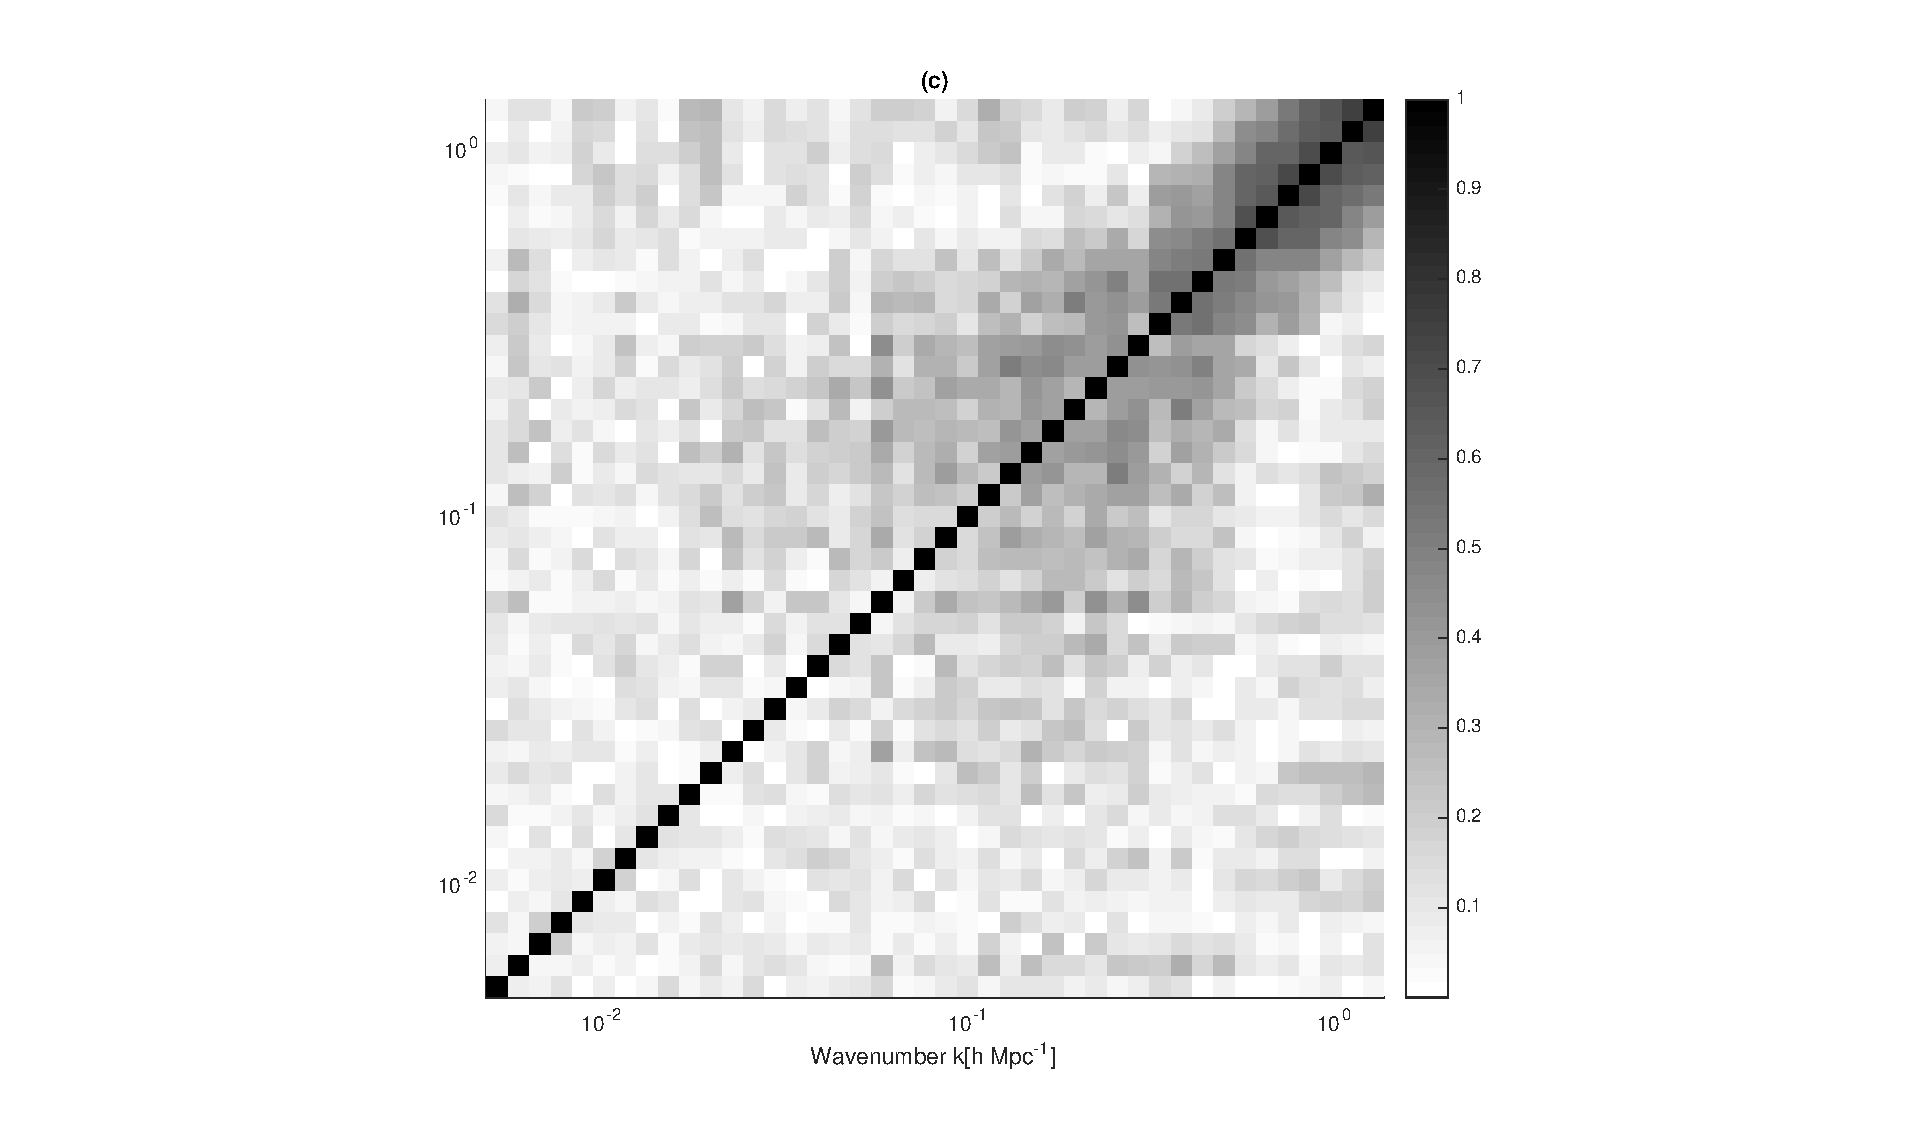
\includegraphics[width=0.5\textwidth]{corrlin.eps}
% \end{subfigure}
%\begin{figure}
%    \centering
%    \includegraphics[width=\textwidth,height=0.5\textwidth]{corrall.eps}
%
  \caption{Cross-correlation coefficient matrix as found from 136 power spectra of the non-linear density field from simulation (the upper triangle) and the deformation potential field from reconstruction(the lower triangle).}   

    \label{fig:corrall}
\end{figure}
    The cumulative, or Fisher, information function of $k_n$ is then defined as the sum of the elements of inverse of subsection of the normalized covariance matrix up to $k_n$ scale
\begin{align}
    I \left( < k_n\right) = \sum_{i,j=1}^n \left[ C^{-1}_{norm} \left( k_i,k_j \right)\right] \left( i,j \leq n \right),
\end{align}
where $C_{norm}$ is the normalized covariance matrix, defined as
\begin{align}
    C_{norm} \left( k,k' \right)=\frac{\mathrm{Cov}(k,k')}{\langle P(k)\rangle\langle P(k)\rangle}.
\end{align}
  
%  The signal-to-noise ratio, sometimes also called Fisher information, can be given by the inverse matrix of covariance. Since the signal-to-noise ratio was given in some work, we also present it for a better comparison. 
%\begin{align}
%\left( \frac{S}{N}\right)^2 (k_{n}) =\sum_{i,j=1}^n P_i \mathrm{Cov}^{-1}(i,j) P_j
%\end{align}
As seen above, cumulative information is a measurement of the number of independent Fourier modes presented in a field up to a given $k_n$, which represents how linear a field is. We plot the cumulative information of the power specta of density fields from simulations and deformation potentials from reconstructions in Fig.\ref{fig:fisherinfo}. In the translinear regime, where $k\sim0.1$, the cumulative information of the non-linear density field has a flat plateau. It indicates that there's nearly no independent information in the translinear regime of the power spectrum. At $k\sim0.8$, the information increase slightly aggain. But the information curve of the reconstructed deformation potential keeps incresing and reaches it's plateau at $k\sim0.6-0.7$ up to a factor of 20. It indicates that APM method can strongly recover the lost information within this scale. 
\begin{figure}[htbp]
 \begin{center}
  \includegraphics[width=0.5\textwidth]{fishernew-crop.pdf}
   \caption{Cumulative information in the power spectra as a function of wavenumber. The blue cycles correspond to the non-linear density field by simulation; the black squares correspond to the the reconstructed deformation potential; the red dash line corresponds to linear density field at $z=0$; the green crosses correspond to linear density field at $z=100$.}
  \label{fig:fisherinfo}
 \end{center}
\end{figure}


\end{section}


\begin{section}{Conclusion}
  \label{sec:conclusion}
  We have considered neutrinos as a dispersive fluid and found that
  this provides additional physical insights into their clustering
  behaviour.  We have computed the sound speed and shown that it
  depends on the intial neutrino velocity distribution and also the
  non-linear cold dark matter.  We find that the excess in power
  observed in the N-body neutrino power spectrum compared to linear
  response can be explained via a higher-order modification to the
  sound speed.  Based on this, we have provided a simple model for the
  neutrino power spectrum that requires no additional integration
  beyond standard Boltzmann code outputs.  Finally, we speculate that
  treating neutrinos as a dispersive fluid could allow for them to be
  simulated efficiently in both memory and processing time.
\end{section}

%\acknowledgements{
  \label{sec:acknowledgements}
  We thank Homg-Ming Zhu and Wang Xin for friendly and helpful discussion.  Computations were performed on
  the General Purpose Cluster supercomputer at the SciNet HPC
  Consortium.  SciNet is funded by: the Canadian Foundation for
  Innovation under the auspices of Compute Canada; the Government of
  Ontario; Ontario Research Fund - Research Excellence; and the
  University of Toronto.  
}


%\bibliographystyle{apsrev}
%\bibliography{thebib}
\widetext
\clearpage
%\input{./supplement.tex}

\end{document}
